\chapter{Somatic Mutation Pipeline for Large-Scale Genomic Data Harmonization}
\label{chap:mut-pipeline-qc}

% Somatic mutation QC report (2018.08)
% https://docs.google.com/document/d/1LW7HBKTwjz3-WCx0j2UedFPSVauulYom2qCbUW3Czbw/edit
% Somatic mutation QC Manuscript (2018.12)
% https://docs.google.com/document/d/1lObJXoxlM4t35DfRjGdZ_xJh3d59VuV7b7B1nGwIuy0/edit



\section{Summary}
We present a systematic analysis of the effects of synchronizing a large-scale, deeply characterized, multi-omic dataset to the current human reference genome, using updated software, pipelines, and annotations.
For each of 5 molecular data platforms in The Cancer Genome Atlas (TCGA)---mRNA and miRNA expression, single nucleotide variants, DNA methylation and copy number alterations---comprehensive sample, gene, and probe-level studies were performed, towards quantifying the degree of similarity between the \enquote*{legacy} GRCh37 (hg19) TCGA data and its GRCh38 (hg38) version as \enquote*{harmonized} by the Genomic Data Commons.
We offer gene lists to elucidate differences that remained after controlling for confounders, and strategies to mitigate their impact on biological interpretation.
Our results demonstrate that the hg19 and hg38 TCGA datasets are very highly concordant, promote informed use of either legacy or harmonized omics data, and provide a rubric that encourages similar comparisons as new data emerge and reference data evolve.


\section{Introduction}
Over the course of a decade The Cancer Genome Atlas (TCGA) helped usher in the era of extreme-scale team science, yielding numerous biological insights and many widely cited papers \cite{hutterc_zenklusenjc:CancerGenome2018}. Underlying this progress in understanding the molecular bases of cancer is one of the broadest, deepest, and most integratively characterized biological datasets ever assembled: on the order of 2 petabytes of primary and secondary data, in the form of 84,000 data aliquots from some 11,300 patients across 33 disease studies. Most TCGA samples were originally aligned against the Genome Reference Consortium build GRCh37 (hg19), with a small fraction (from the pilot phase of TCGA) having been aligned against NCBI Build 36.1 (hg18). Since TCGA was initiated, however, the research community has undergone tremendous evolution, not only in the characterization machinery, due to the enormous drop in sequencing costs, but also in the surrounding ecosystem of reference data, sequence alignment methods, variant calling tools, RNA quantification methods, quality controls used to help distinguish signal from noise, and analysis software. For this reason, the Genomic Data Commons (GDC, \url{https://gdc.cancer.gov/}) was conceived by the National Cancer Institute (NCI) as more than just a massive warehouse of digitized samples: instead, by harmonizing those samples to a uniform reference alignment and gene annotation, then characterizing samples with established tools in consistent workflows and providing updates at regular intervals, the GDC also helps navigate an orderly course through this sea of constant change. The GDC thus offers promise as a force-multiplier for researchers, who can now spend more time exploring their biological questions and less on resolving inconsistencies in data and software versions.

In this paper, we examine the results of the first major harmonization effort undertaken at the GDC: in which the corpus of legacy TCGA data was either aligned or lifted over to the GRCh38 build (hg38) with a GDC workflow assembled from updated versions of bioinformatic tools and reference files used by sequencing and characterization centers in TCGA. While the mechanics of evaluation varied for each data platform, owing largely to natural differences between them and/or how their hg19 counterparts were harmonized to hg38 (e.g., re-alignment of single nucleotide variants [SNVs] versus liftover of SNP6 copy number arrays), in each case \enquote{the aim was to categorize observed differences in analytic results as a function of their sources and control for such to discern potential impact upon biological interpretation.} The sources of variation are given in a figure for each platform and include, among others: (1) genome reference; (2) gene annotation: e.g. UCSC genes, GENCODE, miRBase; (3) upstream methods used in alignment, variant calling and quantification, including: BWA \cite{lih_durbinr:BWAShortRead2009}, STAR \cite{dobina_gingerastr:STARUltrafast2013}, RSEM \cite{lib_deweycn:RSEMAccurate2011}, FPKM-HTSeq \cite{anderss_huberw:HTSeqPython2015}, and MuTect \cite{cibulskisk_getzg:SensitiveDetection2013}; (4) downstream methods used in clustering, correlation, or significance analysis, such as GISTIC \cite{mermelch_getzg:GISTIC2Facilitates2011}; (5) parameterizations such as: thresholds for filtering, p-values or q-values; and (6) auxiliary data, such as: GISTIC marker files and CNV lists, or panels of normals used to remove suspect SNVs. In the interest of reproducibility, the supplement describes the software codes and parameterizations used to carry out these studies, and for each platform includes manifests of the input files upon which our analyses were executed. In the remainder of the text we use the terms ``legacy data'' and ``harmonized data'' interchangeably with ``hg19 data'' and ``hg38 data'', respectively.


\section{Results}

\subsection{Somatic mutations calling pipeline}
TCGA somatic mutation data were generated by whole-exome sequencing in which exome capture was performed using the Agilent SureSelect Human All Exon kit. During TCGA, multiple sequencing platforms (Illumina and SOLiD) were employed. As described in \fref{fig:mut-call-qc-pipeline-comparison}, the analysis pipeline for calling hg38 somatic mutations at the GDC differs substantially from that for calling hg19 somatic mutations in TCGA legacy version (i.e., multi-Center Mutation Calling in Multiple Cancers; MC3 \cite{ellrottk_tcga:MC3MutationCalling2018}).

\begin{figure}[tbp]
    \centering
    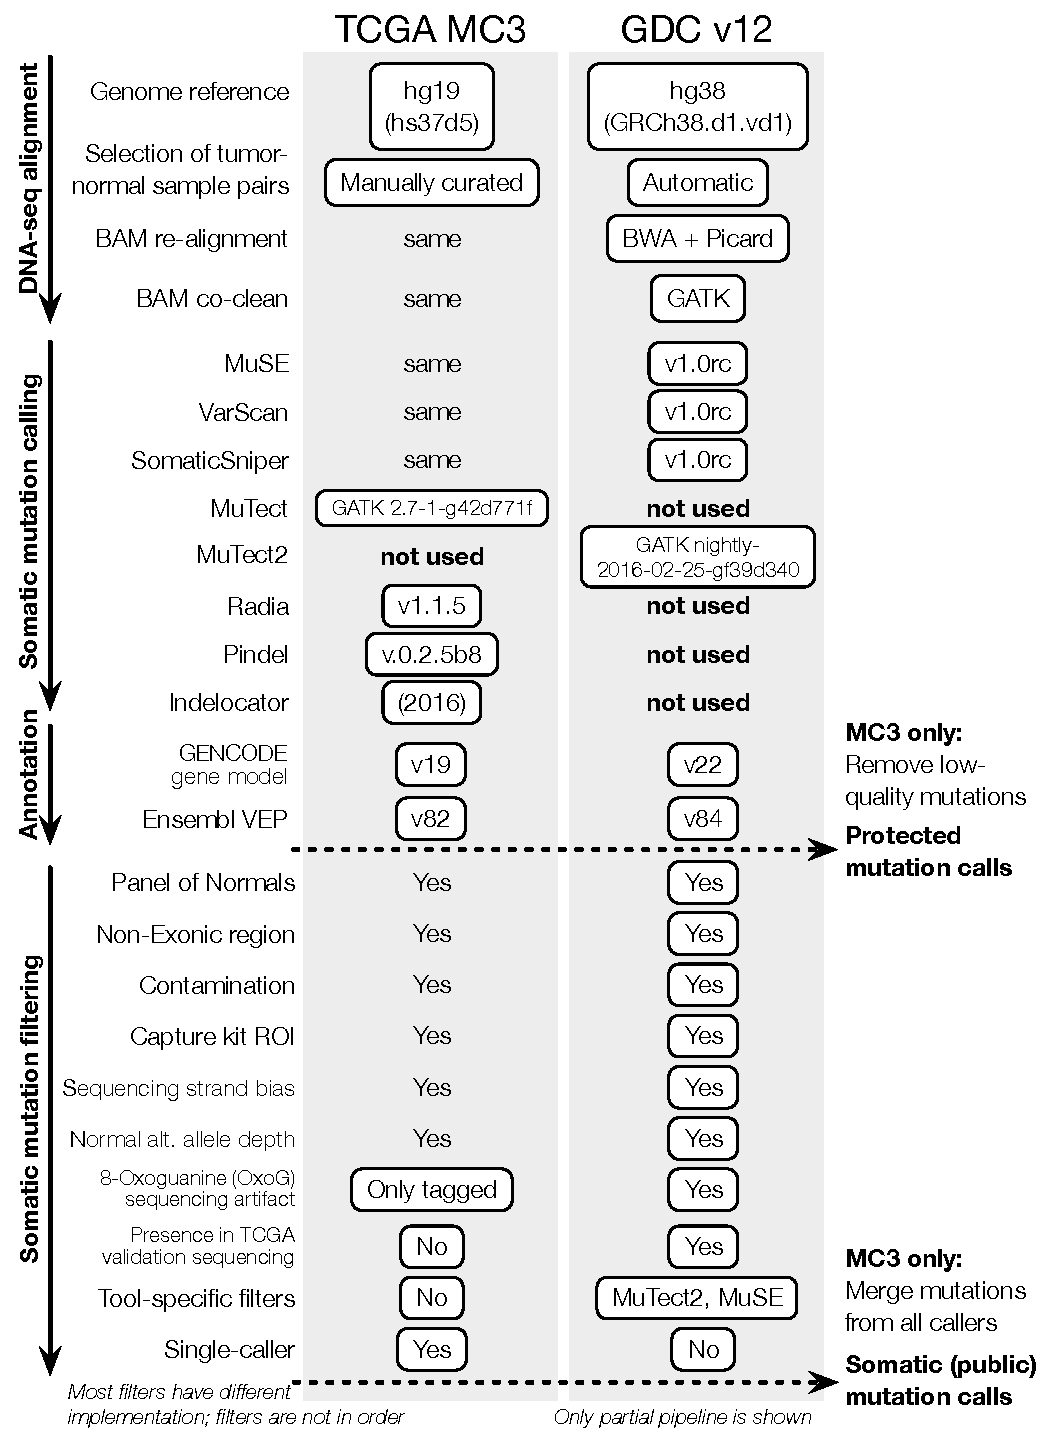
\includegraphics[height=0.9\textheight]{figures/chap02_mutation_pipeline_qc/mutation pipeline difference.pdf}
    \caption{Comparison of the mutation calling pipelines for TCGA MC3 (hg19) and GDC (release v12; hg38).}
    \label{fig:mut-call-qc-pipeline-comparison}
\end{figure}

Although both pipelines used a multiple-caller strategy, there are still some differences---in the processing of alignment files, versions of mutation callers, mutation filters, and gene annotations (\fref{fig:mut-call-qc-pipeline-comparison})---between the MC3 (hg19) and GDC (hg38) mutations.
To characterize those differences and evaluate concordance with prior results, we compared the public somatic mutation calling of single nucleotide variations (SNVs) on multiple TCGA cohorts, using 2,069 samples from the breast, leukemia, colorectal and ovarian cancer cohorts (BRCA, LAML, COAD and OV). We also investigated the `protected' somatic mutation calls of the two groups, which represented the pre-filtered calls. A protected call was excluded from the public call set if it was considered low quality or potentially germline by the filters. GDC protected calls collected all the raw somatic mutation calls detected by all the callers, while MC3 counterpart excluded some low-confidence calls from the raw somatic calls.

The overlap between GDC hg38 and MC3 hg19 mutation calls was calculated by matching their genomic locations and tumor alleles. Across 1,902 shared tumor samples, the mutation overlap between GDC and MC3 contained a total of 488,138 public somatic SNV calls from 21,535 genes (\fref{fig:mut-call-qc-venn-diagram}). The two groups shared 386,350 SNVs (79\%), leaving 71,967 GDC-unique calls and 29,821 MC3-unique calls. We thought the protected somatic calls of one group should represent the universe of all confident somatic mutations; however, there were 45,773 GDC-unique calls and 7,419 MC3-unique calls that the other group could not recover. Those unrecoverable unique calls (21\%) implied that the raw mutation calling from the two groups have different characteristics, so those calls were only reported by the mutation callers in one group (\fref{fig:mut-call-qc-supp-unrecoverable-unique-calls-gdc}, \subcaptionref{fig:mut-call-qc-supp-unrecoverable-unique-calls-mc3}).

\begin{figure}[tb]
    \centering
    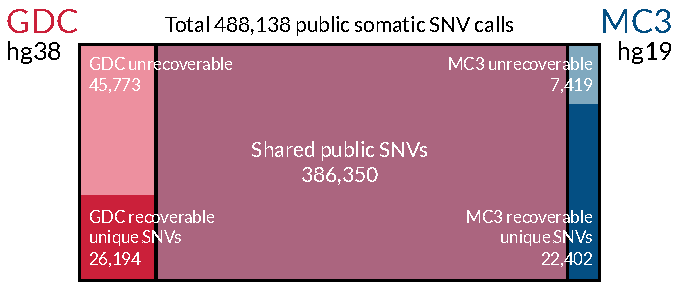
\includegraphics[width=0.9\linewidth]{figures/chap02_mutation_pipeline_qc/overlap_venn_diagram.pdf}
    \caption[Overlapping somatic mutation calls between GDC and MC3.]{Overlapping somatic mutation calls between GDC and MC3. Red and blue shaded regions represent the public somatic SNV calls unique in GDC and MC3, respectively. The lighter red and blue shaded regions represent the unrecoverable calls that were available in the public call of one group but were not found in neither public nor protected calls of the other group.}
    \label{fig:mut-call-qc-venn-diagram}
\end{figure}

\begin{figure}[tbp]
    \centering
    \phantomlabel{fig:mut-call-qc-supp-unrecoverable-unique-calls-gdc}
    \phantomlabel{fig:mut-call-qc-supp-unrecoverable-unique-calls-mc3}
    \phantomlabel{fig:mut-call-qc-supp-gene-model-CCDC168}
    \phantomlabel{fig:mut-call-qc-supp-gene-model-EFCAB8}
    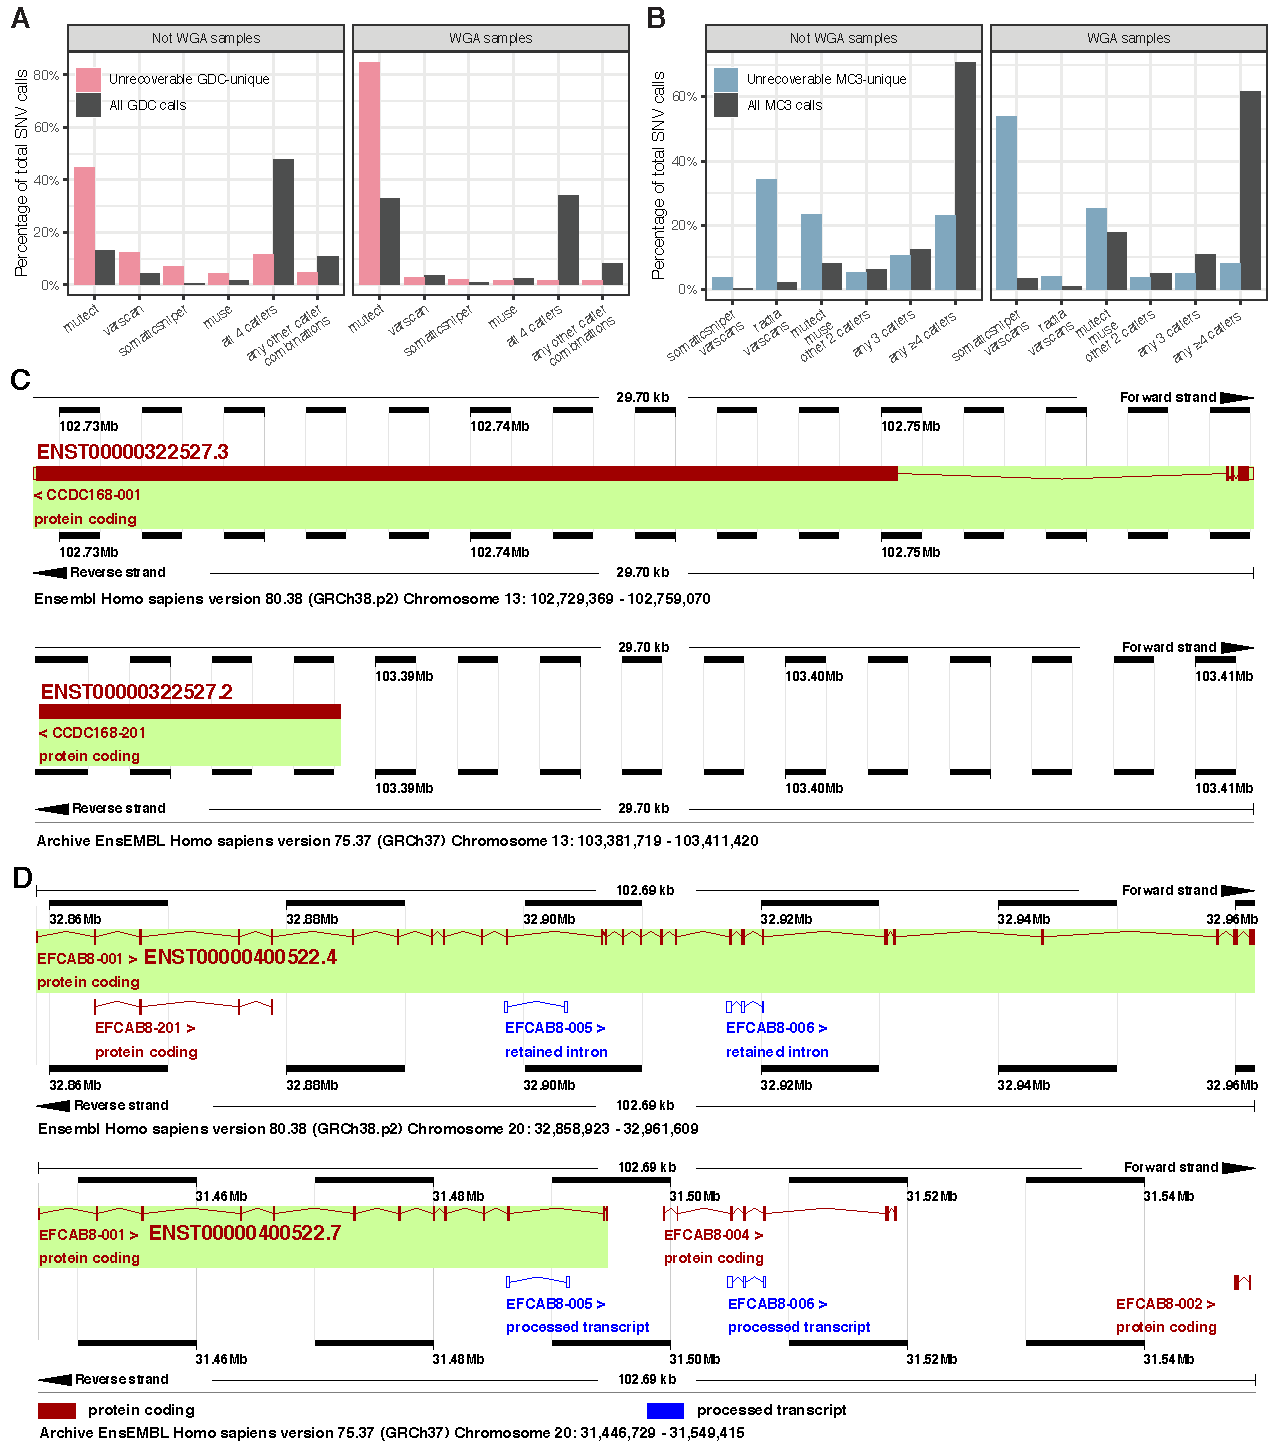
\includegraphics[width=\linewidth]{figures/chap02_mutation_pipeline_qc/supp_figure_combined.pdf}
    \caption{%
        Distribution of mutation caller combinations supporting the unrecoverable unique somatic  mutation calls in \subref{fig:mut-call-qc-supp-unrecoverable-unique-calls-gdc} GDC and \subref{fig:mut-call-qc-supp-unrecoverable-unique-calls-mc3} MC3.
        Gene model comparison of the same transcript in two genome builds. Two genome builds were aligned and displayed in Ensembl genome browser (top: hg38; bottom: hg19):
        \subref{fig:mut-call-qc-supp-gene-model-CCDC168} \gene{CCDC168} (\texttt{ENST00000322527}).
        \subref{fig:mut-call-qc-supp-gene-model-EFCAB8} \gene{EFCAB8} (\texttt{ENST00000400522}).
    }
    \label{fig:mut-call-qc-supp}
\end{figure}

\subsection{Recoverable unique calls reported by GDC}
We then analyzed the recoverable unique calls to investigate how different filtering strategies affected the generation of the public calls from the protected calls. The GDC reported 26,194 recoverable unique calls (the dark red region in \fref{fig:mut-call-qc-venn-diagram}).

First, we identified that the stringent one-caller constraint in MC3 contributed to the majority of the discrepancy between GDC and MC3 call set. MC3 protected 15,478 of those calls (59.0\%) using the one-caller constraint, i.e., the calls were reported by only one MC3 caller. 13,291 of them had no filter in both groups, a sign for good quality calls. Since MC3 labels all one-caller variants to be protected, the constraint might reduce its sensitivity to call true variants.

Among the remaining GDC unique recoverable calls (n = 10,716), 9,475 of them had \texttt{NonExonic} filter in MC3 (36.2\% of all GDC recoverable). The majority of the non-exonic calls in MC3 (n = 8,902; 94.0\%) were also non-exonic in GDC based on the variant classification, including 262 splicing related variants. We found that MC3 and GDC have a different implementation of their \texttt{NonExonic} filter. Those non-exonic calls did not have the \texttt{NonExonic} filter in GDC since they overlapped with an exon from other annotations. Note that the overlapping annotations may be a different gene to what the variant call was annotated, which can be misleading to the users. On the other hand, in MC3, the \texttt{NonExonic} filter relies on the single annotation assigned to a variant call. The implementation difference of the \texttt{NonExonic} filter explained all the variant calls that are non-exonic in two groups. We suggested GDC to either modify the current behavior of the \texttt{NonExonic} filter or document the implementation detail.

Interestingly, we found 573 non-exonic calls in MC3 that were exonic in GDC (2.1\% of all recoverable GDC-unique calls), suggesting those calls were assigned different gene annotations between two groups. For example, we identified two genes (\fref{fig:mut-call-qc-supp-gene-model-CCDC168}, \subcaptionref{fig:mut-call-qc-supp-gene-model-EFCAB8}), \gene{CCDC168} and \gene{EFCAB8}, that have different gene models in different GENCODE versions (MC3: v19; GDC: v22). We have not conducted a systematic check of gene model changes across genome builds, since the affected variant calls are minor compared to other factors mentioned in the report. However, we believe that a comparison of gene models should be released independently to this report, which might be useful for other studies as well. The change can be systematically detected by comparing the transcript ID versions between two annotations.

The choice of Panel of Normal (PoN) samples also altered the inclusion of somatic calls. 1,152 out of 1,241 remaining GDC unique recoverable calls had \texttt{broad\_PoN\_v2} filter in MC3 (4.4\% ). GDC and MC3 may select a different set of PoN samples, though the full list of the PoN samples were unavailable in their documentation.

Lastly, usage of validation sequencing could also alter the somatic status of a variant call. The GDC labels a mutation call `public' when it is also found in the validation sequencing, regardless of the filter status, whereas MC3 calling did not utilize validation status. We identified that the remaining recoverable GDC-unique calls (n = 89) had the capture kit filter \texttt{bitgt} in MC3. Those calls were located in the non-targeted genomic regions of all the capture kits in use, which imply a low read coverage or an incorrect read alignment. They were included in the GDC call set since them were also found in the validation sequencing.


\subsection{Recoverable unique calls reported by MC3}
MC3 reported 22,402 recoverable unique calls (the dark blue region in \fref{fig:mut-call-qc-venn-diagram}), implying those calls were filtered differently in two groups. By following the GDC documentation for somatic MAF file generation, we were able to identify the specific filtering stage where each mutation call was `protected'.

At stage 1 of the GDC filtering, 339 MC3 recoverable unique calls (1.5\% of all recoverable MC3-unique calls) were protected for having \texttt{nonselectedaliquot} or \texttt{multiallelic} filter. GDC and MC3 adopted different sample selection algorithms, which might cause some variant calls to have the texttt{nonselectedaliquot} filter due to a different tumor-normal pair in use for variant calling. MC3 did not implement the \texttt{multiallelic} filter, though we expect very few calls to be affected by this filter due to its low occurrence.

A majority of the variant calls were protected at stage 3 of the GDC filtering (n = 21,681; 96.8\%) for having filters other than \texttt{PASS} and \texttt{panel\_of\_normals} in the \texttt{FILTER} column. We identified a few filters of high occurrence, including `\texttt{t\_lod\_fstar}' filter for MuTect2 calls of low quality (n = 9,366; 41.8\%), `\texttt{bSeq}' reported by DKFZ Bias Filter for all calls with supporting reads biased toward forward or backward strand (n = 6,787; 30.3\%), `\texttt{oxog}' filter provided by D-ToxoG \cite{costellom_getzg:DiscoveryCharacterization2013} for OxoG artifacts (n = 3,626; 16.2\%), all `\texttt{Tier*}' filters for MUSE calls of poor evidence (n = 10,127; 45.2\%), and `\texttt{clustered\_events}' filter for MuTect2 calls located at a reassembled haplotype with too many variants (n = 3,016; 13.5\%). OxoG filter was implemented by both groups but was not used in MC3 for filtering. 3,262 out of 3,626 mutation calls with OxoG filter in GDC also had \texttt{OxoG} filter in MC3 (90\%), implying a good concordance of the filter implementation.

The remaining 382 recoverable MC3-unique calls were protected in the later stages of the GDC filtering: 116 variant calls have at least one of the GDC filters: \texttt{NonExonic} (n = 16), \texttt{bitgt} (n = 30), and \texttt{gdc\_pon} (n = 78). Those filters were also applied in MC3 but those calls did not receive the filter due to change in the gene model definition, different definition of the capture kit set and lift over issue, or different set of PoN samples. The rest of the 266 calls have been reported in the NCBI dbSNP and thus were protected in GDC. In MC3, the ExAC database was used instead for the similar purpose.

In summary, we identified that filters in \texttt{FILTER} column of the GDC MAFs can explain the majority of the recoverable MC3-unique calls (96.8\%). Our analysis left 1 mutation calls unexplained and required further investigation.


\subsection{Mutation calling concordance per sample}
To understand whether the overlap between GDC hg38 and MC3 hg19 somatic mutation calls varies across different samples and cancer types, we calculated the proportion of shared calls over all GDC and MC3 somatic calls for every sample (\fref{fig:mut-call-qc-overlap}). Overall, we observed that different cancer types exhibited very different levels of concordance. COAD samples had the largest fraction of concordant calls, where 243 out of the total 376 samples (88\%) had a higher shared call percentage than the median in both GDC and MC3. In contrast, LAML samples exhibited the worst concordance between the two groups, which may be due to this cohort having incomplete demultiplexing, and using Whole Genome Amplification (WGA) in library construction \cite{bodinim_rival:HiddenGenomic2015}.

\begin{figure}[tb]
    \centering
    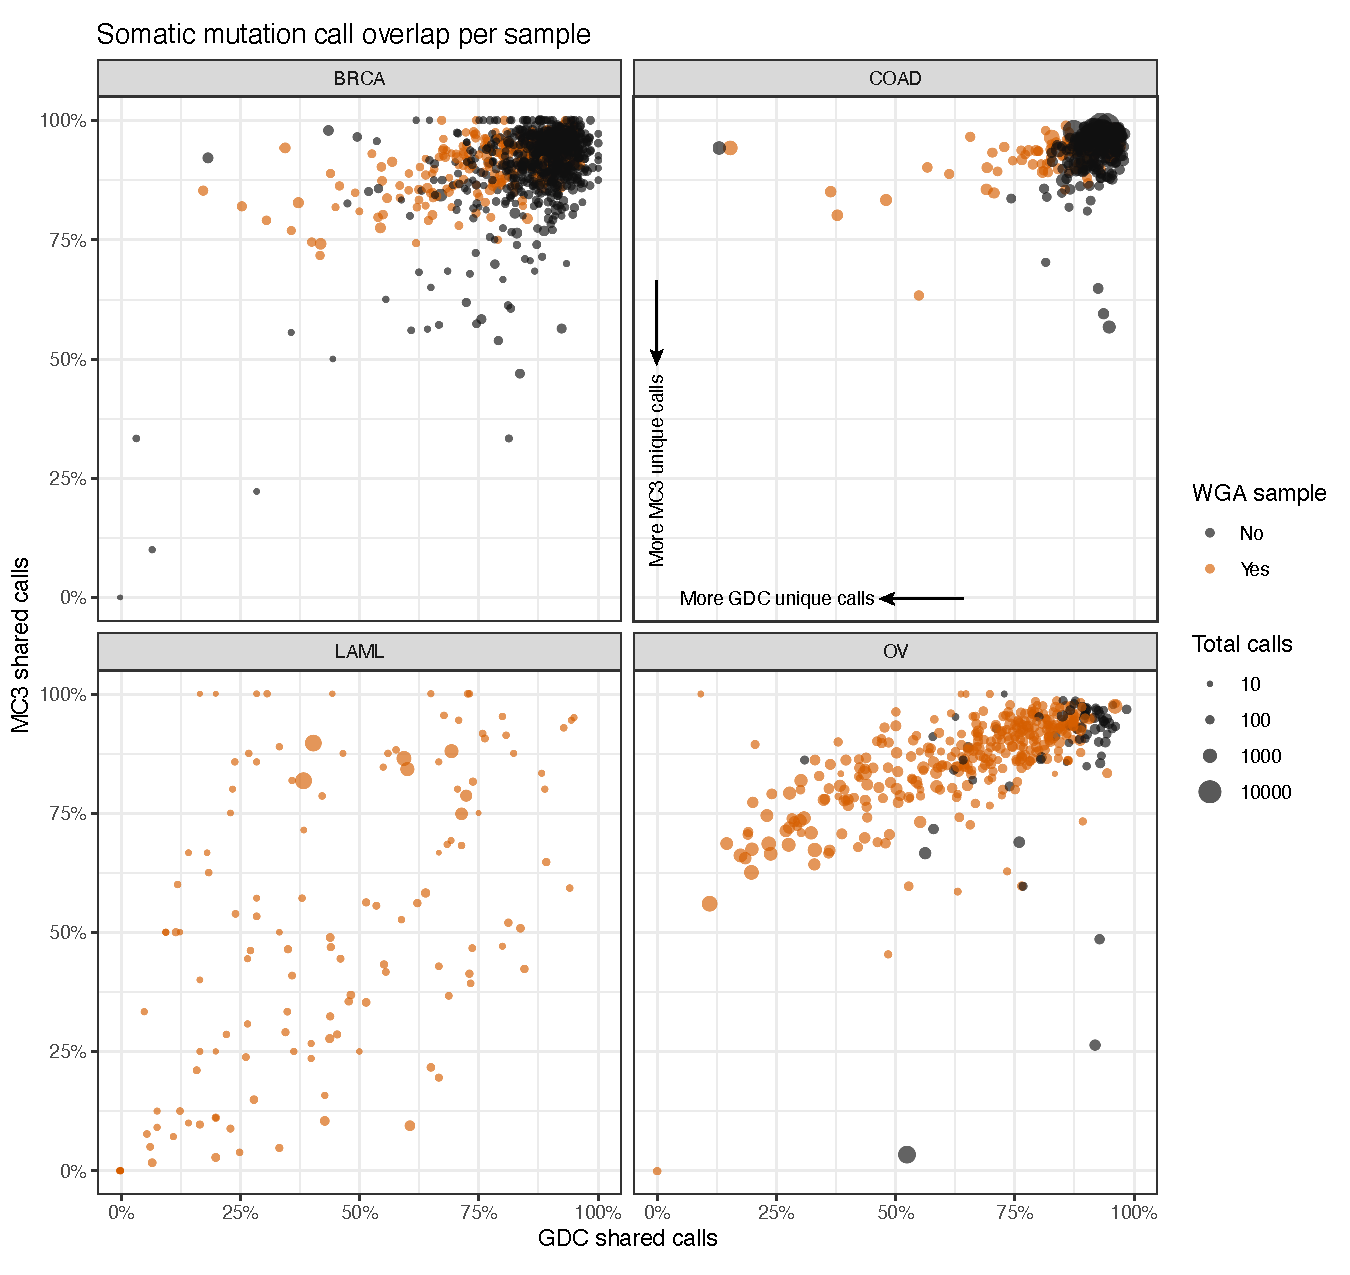
\includegraphics[width=0.9\linewidth]{figures/chap02_mutation_pipeline_qc/GDC_MC3_overlap_per_sample.pdf}
    \caption[Overlapping somatic mutation calls between GDC and MC3 per sample.]{The overlap of somatic mutation call per sample in four different cancer types. The X and Y axes represent the proportion of shared calls over the total calls from GDC and MC3 respectively. Each dot represents a sample, and the dot size indicates the numbers of somatic SNVs called. A sample has more GDC-unique or MC3-unique calls is closer to the origin. The color indicates whether WGA sequencing was employed. See also \fref{fig:mut-call-qc-supp}.}
    \label{fig:mut-call-qc-overlap}
\end{figure}

From our analysis, we found that 79\% of all the public somatic mutation calls from two groups were concordant. When we excluded LAML samples, 80\% of all the public somatic calls were concordant, and the average of the fraction of concordant calls per sample improved from 72.5\% to 75.9\%. We were able to explain the remaining non-concordant public mutation calls by the three major sources of the differences: for unrecoverable unique calls, mutation caller; for recoverable unique calls, filtering strategy and gene annotation version. The detailed list of the non-concordant mutation calls and explanation is available at \url{https://gdc.cancer.gov/about-data/publications/HG38QC}.


\section{Discussion}
The publication of the first human reference genome unleashed a torrent of cancer research, in which the field witnessed a steady transition from a largely qualitative and wet lab-based practice to one that is far more quantified and digital. While TCGA has played important catalytic and leadership roles in this transformation, the resulting increase in volume and complexity of data are pushing the limits of our capacity to store, process and make sense of it. At the same time, characterization and software technologies, analytic methods and reference data continue to rapidly evolve. The cumulative effect of these forces---size, complexity, and accelerated change---mean researchers have to confront substantial technical and logistical challenges before they can begin to ask basic biological questions.

This study helps address those challenges, and is important to the research community in several ways: (i) Scientifically, because confidence in and usability of global resources like TCGA must remain high even as the data they offer and fields they serve experience enormous growth and change. Findings published from such resources, which purport to describe fundamental biology, should remain evident no matter how the primary data are transformed after original collection; and any findings refuted after such transformations should be revised or discarded. By demonstrating significant concordance between the legacy hg19 and GDC-harmonized hg38 versions of TCGA data, our study girds the corpus of TCGA-related research and suggests it will continue to play a valuable role into the foreseeable future. (ii) Technologically, because the GDC will play an important role in the usability of many large data sets beyond TCGA---e.g. TARGET and others which are currently generating data---and in offering these data to the world the GDC has updated or introduced new data models, ontologies, back-end infrastructure as well as front-end portals and APIs. When combined with the fact that many of the scientific algorithms and knowledge bases used to generate legacy TCGA data have either evolved or been superseded, this means that the number of moving parts—and therefore the sources of potential variation—in the harmonized hg38 data served by the GDC, is high. The work reported here isolates confounding factors in the technology stack for each platform, offers sets of outliers for each platform, and indicates that TCGA results should be relatively insensitive to changes between legacy hg19 and harmonized hg38 data processing. (iii) Efficiency and cost-effectiveness, because the scope of the vetting effort reported here would be impractical for many labs or academic departments to conduct themselves prior to confidently utilizing GDC data in their work. Our study provides a framework that may guide similar comparative analyses in the future, online resources for follow-up exploration, and tools that can be hardened, generalized, and deployed to form the basis of future QC efforts in other large-scale projects.


\section{Methods}
Throughout the decade that spanned the TCGA project, somatic mutation calling has been constantly improved and all the accumulated knowledge was recently applied to a harmonized set of mutation calls across all TCGA samples: the Multi-Center Mutation Calling in Multiple Cancers (MC3) project, as a part of the TCGA Pan-Cancer Atlas effort. The unified MC3 somatic mutations were called using standardized protocols and annotated with various filters to detect potential sequencing artifacts and label low quality variant calls. Two centers, DNAnexus and FIREHOSE, generated somatic mutation calls for each pipeline (7 tools) on each sample (> 10,000 tumor-normal pairs), from 33 cancer types \cite{ellrottk_tcga:MC3MutationCalling2018}. The tool developers supplied the identification of tool-specific, sample-specific, and mutation-specific filters. The filter flags were present in a comma separated column which were carried through to the mutation annotation file (MAF). These mutation calls supply the basis for many PanCancer Atlas analysis working groups.

Despite the uniformity, the MC3 pipeline was designed for the human genome reference hg19. On the other hand, GDC has developed a different somatic mutation calling pipeline for a newer human genome reference version, hg38. The GDC pipeline was designed to be fully automatic. Therefore, whenever an algorithm of variant calling or filtering gets improved, GDC can generate an updated set of uniform variant calls across all samples by updating the data release version.

To understand the differences introduced by the genome build change and the pipeline implementation, we compare the somatic mutation calls of samples from four TCGA cancer types. The choice of these four cancer types was to provide a good presentation of possible attributes contributing to the outlier status, including the library construction, sequencing technology, sequencing center, and the mutation rate.

\subsection{Data Source}
GDC MAFs in hg38 were obtained through the GDC Data Portal. GDC version 12.0 was used, which was released in June 2018. The query for the file retrieval was:

\par\noindent\begin{verbatim}
    cases.project.project_id
    in ["TCGA-LAML", "TCGA-BRCA", "TCGA-COAD", "TCGA-OV"]
    and files.data_format = "MAF"
\end{verbatim}

The query returned both somatic and protected MAFs, totaling 32 files and covering 2,069 tumor and paired normal samples. Note that protected somatic mutation calls did not reflect the full pool of germline variants. Protected MAFs contained the raw mutation calls from all somatic mutation callers. Each protected MAF underwent various filters to remove calls of low quality or potential germline variants reported in the germline variant databases like dbSNP \cite{sherryst_sirotkink:dbSNP2001} and Exome Aggregation Consortium (ExAC) \cite{lekm_exomeaggregationconsortium:AnalysisProteincoding2016}. Germline variant calling used a different algorithm, thus not all the germline variants would be captured in the protect MAFs, which is beyond the scope of our study.

TCGA MC3 MAFs were obtained from Synapse (somatic: syn7214402; protected: syn5917256). The genomic coordinates of MC3 variant calls were lifted over from hg19 to hg38 using CrossMap v0.2.7 and chain files from University of California, Santa Cruz (UCSC). Variant calls that could not be lifted over were dropped and excluded from our analysis. Among the four cancer types, 1,902 samples that had somatic mutation calls from both MC3 and GDC were used for the rest of the comparison.

\subsection{Mutational Calling Pipelines}
The GDC variant calling pipeline of release 12.0 was described as follows: the pipeline started with genome re-alignment to GRCh38.d1.vd1 by extracting sequencing reads from a sample's BAM files using Biobambam. The re-aligned BAM files were merged and cleaned up using Picard and GATK. Four tools were used for the variant calling: MuSE, MuTect2, VarScan2, and SomaticSniper. MuTect employed a ``Panel of Normals'' (PoN) to reduce the rate of germline variant call and, more often, recurrent sequencing artifacts. The PoN was selected from the TCGA blood normal genomes curated to be cancer-free. VarScan and MuTect are also able to generate indel calls, which were collected together with the single nucleotide variant (SNV) calls. Variant calls were annotated using Variant Effect Predictor (VEP) version 84, which was based on GENCODE version 22. Various filters were added to both MAF and Variant Call Format (VCF) files during the annotation. Please refer to the following GDC documentation for more details:

\tightlists
\begin{itemize}
    \tightlist
    \item \href{https://docs.gdc.cancer.gov/Data/File_Formats/MAF_Format/}{File Format: MAF}
    \item \href{https://docs.gdc.cancer.gov/Data/File_Formats/VCF_Format/}{File Format: VCF}
    \item \href{https://docs.gdc.cancer.gov/Data/Bioinformatics_Pipelines/DNA_Seq_Variant_Calling_Pipeline/#somatic-variant-calling-workflow}{Bioinformatics Pipeline: DNA-Seq Workflow--Somatic Variant Calling Workflow}
\end{itemize}
\defaultlists

Complete details of the MC3 variant calling pipeline were provided in the MC3 publication \cite{ellrottk_tcga:MC3MutationCalling2018}, with the key aspects as follows. Non hg19 aligned samples were excluded from the pipeline. Implementation of these tools were performed by DNAnexus including SomaticSniper \cite{larsonde_dingl:SomaticSniper2012}, MuSE \cite{fany_wangw:MuSE2016}, Pindel \cite{yek_ningz:Pindel2009}, Radia \cite{radenbaughaj_hausslerd:RADIA2014}, and Varscan \cite{koboldtdc_wilsonrk:VarScan22012} and by Broad Institute including MuTect \cite{cibulskisk_getzg:SensitiveDetection2013} and Indelocator. Filtering for each tool was provided by the tool developers. Filtered VCFs were merged and converted to MAF. During the conversion, annotations were provided by many databases such as Ensembl version 75, GENCODE v19 using Variant Effect Predictor (VEP) version 82. A Panel of Normals (filter flag: \texttt{broad\_PoN\_v2}) was also used. Sample level annotations were also added to the MAF, including additional filters: \texttt{gapfillter}, \texttt{contest}, \texttt{badseq}, \texttt{nonpreferredpair}, and \texttt{wga}. The MAF file was then split to 2 MAFs. A flagged MAF available to the public, and a protected MAF harboring all mutations that were merged after flagging potential artifacts.

\subsection{Comparative Analysis}
The variant call overlap between GDC and MC3 was done by matching their genomic location and tumor allele 2. To identify the potential causes for the unique calls in the two groups, we investigate the overlap result in the following subsets: unique calls in each group, sample-wise overlap, and recoverable unique calls in each group. To understand whether the overlap between GDC and MC3 calls varies across different samples and cancer types, we calculated the proportion of shared calls over total GDC and MC3 calls for every sample.

\subsection{Code and Data Availability}
The scripts to generate the mutation matching between GDC and MC3 pipelines and conduct all related analyses can be found at \url{https://github.com/ding-lab/gdc_qc_analysis}. All MAF files used in the analysis can be found in \tref{tab:mut-call-qc-data-src}.

\begin{table}[tbp]
    \centering
    \caption{Somatic Mutation MAF file manifests.}
    \label{tab:mut-call-qc-data-src}

    \footnotesize
    \begin{subtable}{1\linewidth}
        \centering
        \subcaption{GDC}\label{tab:mut-call-qc-data-src-gdc}
        \begin{tabular}{lllr}
            \toprule
            Cancer type & Mutation caller & Access & File UUID \\
            \midrule
            BRCA & MuSE & controlled & \texttt{cd0d1636-ae95-4141-94b3-8218eb3b8b25} \\
            BRCA & MuTect & controlled & \texttt{053f01ed-3154-4aea-9e7f-932c435034b3} \\
            BRCA & SomaticSniper & controlled & \texttt{f9ff49e9-31ce-4051-9157-4bf4b0c5859a} \\
            BRCA & VarScan & controlled & \texttt{5a6c3396-8c49-4c25-8a86-7ae63a887c43} \\
            COAD & MuSE & controlled & \texttt{1eabb7b5-66b5-403c-b5ca-d1b83acfad33} \\
            COAD & MuTect & controlled & \texttt{1e560f0b-cbc5-4e50-96b0-c096394acb2b} \\
            COAD & SomaticSniper & controlled & \texttt{08a28aec-5502-4cdc-b668-62b11f8f5bc2} \\
            COAD & VarScan & controlled & \texttt{b453bdde-d1c1-460c-9a70-d87c656f1a7b} \\
            LAML & MuSE & controlled & \texttt{b85b532a-45ae-4510-88f8-11e5bcbe72dd} \\
            LAML & MuTect & controlled & \texttt{66124158-7feb-4b8e-8fc4-393a5e641fea} \\
            LAML & SomaticSniper & controlled & \texttt{5292b256-4db8-49dc-8952-c048a4fe4c5a} \\
            LAML & VarScan & controlled & \texttt{799ea420-6768-42e8-8544-ce7a81ab54fd} \\
            OV & MuSE & controlled & \texttt{1cb59aef-ef3f-4367-9a3d-f33f7fb93e40} \\
            OV & MuTect & controlled & \texttt{e6ea3b5e-48fc-4155-81f6-4ffe59871d5a} \\
            OV & SomaticSniper & controlled & \texttt{4683fdc3-2041-4b03-9886-fd035ab64c4f} \\
            OV & VarScan & controlled & \texttt{04da990e-67a3-4ead-ab08-448c7118624c} \\
            BRCA & MuSE & open & \texttt{b8ca5856-9819-459c-87c5-94e91aca4032} \\
            BRCA & MuTect & open & \texttt{995c0111-d90b-4140-bee7-3845436c3b42} \\
            BRCA & SomaticSniper & open & \texttt{7dd592e3-5950-4438-96d5-3c718aca3f13} \\
            BRCA & VarScan & open & \texttt{6c93f518-1956-4435-9806-37185266d248} \\
            COAD & MuSE & open & \texttt{70cb1255-ec99-4c08-b482-415f8375be3f} \\
            COAD & MuTect & open & \texttt{03652df4-6090-4f5a-a2ff-ee28a37f9301} \\
            COAD & SomaticSniper & open & \texttt{70835251-ddd5-4c0d-968e-1791bf6379f6} \\
            COAD & VarScan & open & \texttt{8177ce4f-02d8-4d75-a0d6-1c5450ee08b0} \\
            LAML & MuSE & open & \texttt{0cdf3c70-ad58-462d-b6ba-5004b26c618e} \\
            LAML & MuTect & open & \texttt{27f42413-6d8f-401f-9d07-d019def8939e} \\
            LAML & SomaticSniper & open & \texttt{99c2a8ba-1930-4dc7-ad71-7883eb7e29a9} \\
            LAML & VarScan & open & \texttt{e595f93d-41ac-435e-8c90-06df7e9d6742} \\
            OV & MuSE & open & \texttt{51423d79-e9c5-4c4d-b12c-99c1338dbd43} \\
            OV & MuTect & open & \texttt{b22b85eb-2ca8-4c9f-a1cd-b77caab999bd} \\
            OV & SomaticSniper & open & \texttt{3e48014d-ce4a-4937-bba4-13eaf631a64a} \\
            OV & VarScan & open & \texttt{a8f41106-633d-4027-9e1f-e73bfd48f11e} \\
        \bottomrule
        \end{tabular}
    \end{subtable}

    \vspace{\baselineskip}

    \begin{subtable}{1\linewidth}
        \centering
        \subcaption{MC3}\label{tab:mut-call-qc-data-src-mc3}
        \begin{tabular}{llr}
            \toprule
            Synapse ID & Access & File UUID  \\
            \midrule
            syn7214402 & open & \texttt{1c8cfe5f-e52d-41ba-94da-f15ea1337efc} \\
            syn5917256 & controlled & \texttt{8b851024-2915-4d66-8a84-d03199b616fd} \\
            \bottomrule
        \end{tabular}
    \end{subtable}
\end{table}
